\newappendix{Environment description}
\label{sec:task-renders}


\begin{figure}[h]
\centering
\begin{subfigure}[t]{0.3\textwidth}
    \includegraphics[width=\textwidth]{figures/dyne/ReacherVertical.jpg}
    \caption{\texttt{ReacherVertical}}
\end{subfigure}
\begin{subfigure}[t]{0.3\textwidth}
    \includegraphics[width=\textwidth]{figures/dyne/ReacherTurn.jpg}
    \caption{\texttt{ReacherTurn}}
\end{subfigure}
\begin{subfigure}[t]{0.3\textwidth}
    \includegraphics[width=\textwidth]{figures/dyne/ReacherPush.jpg}
    \caption{\texttt{ReacherPush}}
\end{subfigure}
\caption{The Reacher family of environments. \texttt{ReacherVertical} requires the agent to move the tip of the arm to the red dot. \texttt{ReacherTurn} requires the agent to turn a rotating spinner (dark red) so that the tip of the spinner (gray) is close to the target point (red). \texttt{ReacherPush} requires the agent to push the brown box onto the red target point. The initial state of the simulator and the target point are randomized for each episode. In each environment the rewards are dense and there is a penalty on the norm of the actions. The robot's kinematics are the same in each environment but the state spaces are different.}
\label{fig:reacher_family}
\end{figure}

The first task family, pictured in Figure \ref{fig:reacher_family}, is the ``Reacher family'', based on the \texttt{Reacher-v2} MuJoCo \citep{todorov2012mujoco} task from OpenAI Gym \citep{brockman2016openai}.
These tasks form a simple new benchmark for multitask robot learning.
The first task, which we use as the ``source'' task for training the DynE space, is \texttt{ReacherVertical}, a standard reach to a location task.
The other two tasks are inspired by the DeepMind Control Suite's \texttt{Finger Turn} and \texttt{Stacker} environments, respectively \citep{tassa2018deepmind}.
In \texttt{ReacherTurn}, the same 2-link Reacher robot must turn a spinner to the specified random location.
In \texttt{ReacherPush}, the Reacher must push a block to the correct random location.

\begin{figure}[h]
\centering
\begin{subfigure}[t]{0.3\textwidth}
    \includegraphics[width=\textwidth]{figures/dyne/Pusher.png}
    \caption{\texttt{Pusher-v2}}
\end{subfigure}
\begin{subfigure}[t]{0.3\textwidth}
    \includegraphics[width=\textwidth]{figures/dyne/Striker.png}
    \caption{\texttt{Striker-v2}}
\end{subfigure}
\begin{subfigure}[t]{0.3\textwidth}
    \includegraphics[width=\textwidth]{figures/dyne/Thrower.png}
    \caption{\texttt{Thrower-v2}}
\end{subfigure}

\caption{The 7DoF family of environments. \texttt{Pusher-v2} requires the agent to use a C-shaped end effector to push a puck across the table onto a red circle. \texttt{Striker-v2} requires the agent to use a flat end effector to hit a ball so that it rolls across the table and reaches the goal. \texttt{Thrower-v2} requires the agent to throw a ball to a target using a small scoop.  As with the Reacher family, the dynamics of the robot are the same within the 7DoF family of tasks. However, the morphology of the robot, as well as the object it interacts with, is different.}
\label{fig:7dof_family}
\end{figure}

The second task family is the ``7DoF family'', which comprises \texttt{Pusher-v2}, \texttt{Striker-v2}, and  \texttt{Thrower-v2} from OpenAI Gym \citep{brockman2016openai}.
We use \texttt{Pusher-v2} as the source task.
These tasks use similar (though not identical) robot models, making them a feasible family of tasks for transfer.
They are shown in Figure \ref{fig:7dof_family}.

\subsection{Pixels}
We use full-color images rendered at 256x256 and resized to 64x64 pixels.
In order to allow the agents to perceive motion, we stack the current frame with the three most recent frames, resulting in an observation of dimension 12x64x64.


\newappendix{Hyperparameters and DynE training} \label{sec:hyperparams}

For DynE-TD3 we use all of the default hyperparameters from the TD3 code\endnote{\url{https://github.com/sfujim/TD3}} across all tasks.
For all experiments we choose the dimension of the DynE action space to be equal to the dimension of a single action in the environment.
We set the number of actions in the DynE space to be $k=4$ for all experiments except \texttt{Thrower-v2}, for which we use $k=8$.
We use the Adam optimizer \citep{kingma2014adam} with learning rate $10^{-4}$.
All our experiments used recent-model NVidia GPUs.


\paragraph{Training on states}
When computing log-likelihoods we divide by the number of dimensions in the state in an attempt to make the correct settings of $\gamma$ invariant to the observation dimension; the same result could be achieved by multiplying the values of $\gamma$ that we report by the state dimension and changing the learning rate.
With that scaling we set we set our hyperparameters $\gamma = \lambda = 10^{-2}$ across all environments.
We concatenate all the joint angles and velocities to use as the states during representation learning.
We preprocess the $s, s'$ pairs by first taking the difference $\Delta s = s' - s$ and then whitening so that $\Delta s$ has zero mean and unit variance in each dimension.
This preprocessing encourages the encoder to represent both position and velocity in the latent space; the scales of these two components are quite different.

We use fully-connected networks for the action encoder $e_a$ and the conditional state predictor $f$. Each function has two hidden layers of 400 units.
Training this model should take 5-10 minutes on GPU.


\paragraph{Training on pixels}
We train a DynE model for each environment, taking in a stack of frames and a sequence of $k=4$ actions and predicting future states.
To speed training we predict only the two latest frames of the future state (i.e. the picture of the world at time $t+k$ and $t+k-1$) instead of all four.
When doing RL we take the state encoder $e_s$ from this model and use it to preprocess all states from the environment.

We set the dimension of the state embedding $z_s$ to 100.
We did not try other options, and given the sensitivity of RL to state dimension a smaller setting would very likely yield faster learning.
We set $\beta = \gamma = 1$, at which setting DynE is optimizing a variational lower bound on $p(s_{t+k} | s_t, \va^k)$.
% This number is small due to our rescaling of the log-likelihood by the dimension; without that rescaling it would be $\approx 1$.
% As the goal of this objective is representation learning, not generation, it is better to err on the side of setting $\beta$ and $\gamma$ too small. This results in higher fidelity but lower structure, which is better than low-fidelity but smooth (or constant) latent spaces.
We recommend ensuring that the predictions (not generations) from the model are correctly rendering all the task-relevant objects; if $\beta$ and $\gamma$ are too high, the model may incur lower loss by ignoring details in the image.
We use cyclic KL annealing \citep{liu2019cyclical} to improve convergence over a wide range of settings.

We use the DCGAN architecture \citep{radford2015unsupervised} for the image encoder $e_s$ and the predictor $f$. The action encoder $e_a$ is fully connected with two hidden layers of 400 units. Training this model takes 1-2 hours on GPU.



\newappendix{Varying levels of temporal abstraction}
\label{sec:varying_k}

We study the impact of varying $k$, the level of temporal abstraction in the DynE action space.
We find that increasing $k$ improves performance and learning speed up to a point; beyond this point, performance degrades.
The optimal setting of $k$ will depend on the environment dynamics.
We expect that environments with very slow dynamics will benefit from a greater degree of temporal abstraction.


\begin{figure}[h]
\centering
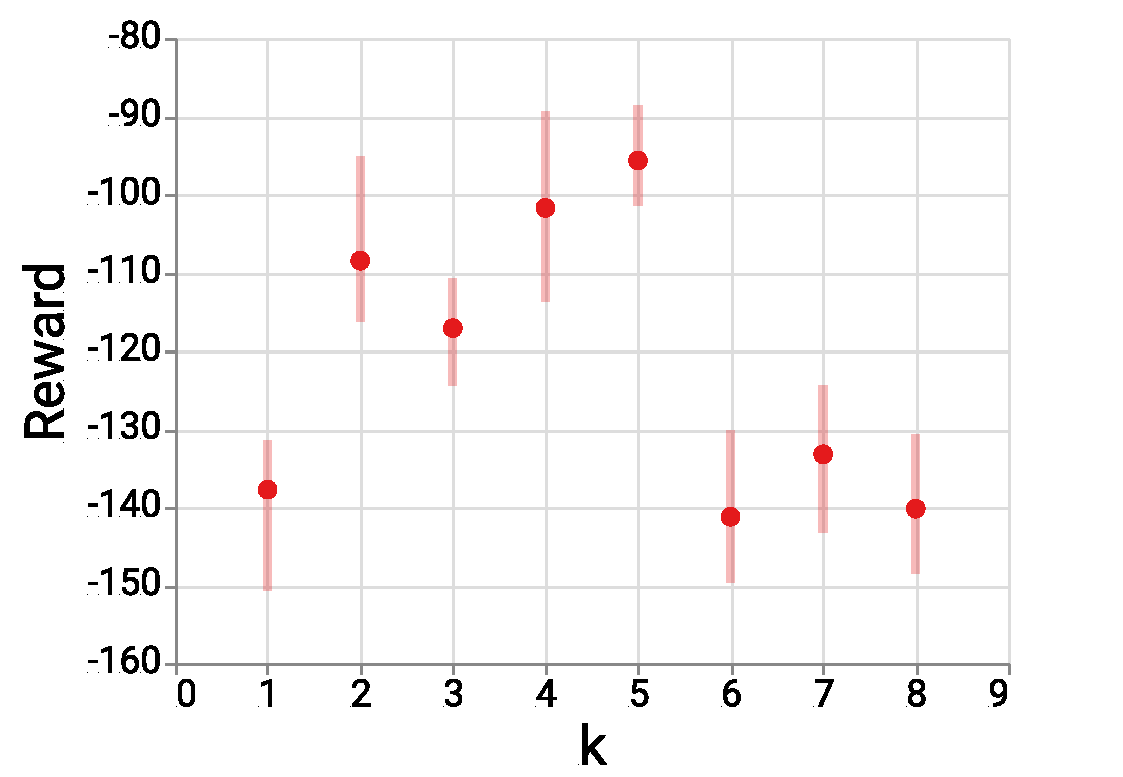
\includegraphics[width=0.5\textwidth]{figures/dyne/varying_k_RP.pdf}
\caption{DynE-TD3 results on Reacher Push with varying $k$.
We find that increased temporal abstraction improves performance up to a point, beyond which the action space is no longer able to represent the optimal policy and performace degrades.
Solid points are the mean reward obtained after training for 1M environment steps. Shaded bars represent the min and max performance over 4 seeds.}
\label{fig:varying_k}
\end{figure}





\newappendix{Visualizing the DynE action space}
\label{sec:latent-vis}

% \red{replace this figure with one about states or clean it up}

To better understand the structure in the DynE action embedding space, we visualize the relationship between the outcome of a sequence of actions and the DynE embedding of those actions.
When embedding an action sequence, the DynE objective seeks to preserve information about the outcome of that action sequence (i.e. the change in state), but minimize information about the original action sequence.
Therefore we should see that all action sequences which have similar outcomes embed close together, regardless of the actions along the way.
% We investigate this by plotting the 2D DynE embedding of 10K action sequences and coloring them by their outcome under the environment dynamics.
% If the DynE embedding depends on the actions within the sequence and not just the outcome, some sequences with similar outcomes (colors) will be embedded far apart.
\Cref{fig:spaces} investigates this in a simple Point environment with an easy-to-visualize 2D $(x, y)$ state.
For this simple problem, we see that all pairs of action sequences $\va^k_1$ and $\va^k_2$ with similar outcomes are close together in the embedding space.
The correspondence between the two spaces appears to remain strong for high-dimensional and nonlinear environments, but is much harder to render in two dimensions.

\begin{figure}[h]
\centering
\begin{subfigure}[t]{0.3\textwidth}
    \includegraphics[width=\textwidth]{figures/dyne/state_space_rainbow.png}
    \caption{Outcome space}
\end{subfigure}
\begin{subfigure}[t]{0.3\textwidth}
    \includegraphics[width=\textwidth]{figures/dyne/latent_space_rainbow.png}
    \caption{DynE action space}
\end{subfigure}
\caption{The mapping between the outcomes and embeddings of action sequences.
We sample 10K random sequences of four actions and evaluate their outcomes in the environment dynamics, measured by $(\Delta x, \Delta y) = s_{t+4} - s_t$.
\textbf{(a)} We plot the outcome $(\Delta x, \Delta y)$ of each action sequence and color each point according to its location in the plot.
\textbf{(b)} We use DynE to embed each action sequence into two dimensions; each point in this plot corresponds to a point in (a) and takes its color from that corresponding point.
The similarity of the two plots and the smooth color gradient in (b) indicate that DynE is embedding action sequences according to their outcomes.
}
\label{fig:spaces}
\end{figure}

\newpage
\newappendix{Extended results}
\label{sec:extended_results}

\begin{figure}[h]
\centering
\includegraphics[width=\textwidth]{figures/dyne/extended_pixel_results.pdf}
\label{fig:extended_pixel_results}
\caption{These plots allow for direct comparison between the methods from pixels (Pixel-TD3, VAE-TD3, S-DynE-TD3, and SA-DynE-TD3) and our baselines from low-dimensional states (PPO and SAC). The DynE methods from pixels perform competitively with some baselines from states.}
\end{figure}

\newappendix{Exploration with raw and DynE action spaces}
\label{sec:exploration_trajs}

\begin{figure}[h]
\centering
\begin{subfigure}[t]{0.45\textwidth}
    \includegraphics[width=\textwidth]{figures/dyne/explore_random.png}
    \caption{Random exploration with raw actions}
\end{subfigure}
\begin{subfigure}[t]{0.45\textwidth}
    \includegraphics[width=\textwidth]{figures/dyne/explore_sto.png}
    \caption{Random exploration with DynE}
\end{subfigure}
\label{fig:exploration}
\caption{These figures illustrate the way the DynE action space enables more efficient exploration. Each figure is generated by running a uniform random policy for ten episodes on a \texttt{PointMass} environment. Since the environment has only two position dimensions, we can plot the actual 2D position of the mass over the course of each episode. \textbf{Left:} A policy which selects actions at each environment timestep uniformly at random explores a very small region of the state space. \textbf{Right:} A policy which randomly selects DynE actions once every $k$ timesteps explores much more widely.}
\end{figure}


\printendnotes